\documentclass[tikz,border=4pt]{standalone}
\usepackage[T1]{fontenc}
\usepackage{lmodern}
\usepackage{amssymb}
\usetikzlibrary{positioning,fit,calc,arrows.meta,shapes.misc,shapes.geometric,backgrounds}

% Exact palette from ../inferencex_overview.py (including its inline blue).
\definecolor{INK}{HTML}{1f2937}
\definecolor{MUTED}{HTML}{6b7280}
\definecolor{PANEL}{HTML}{f5f5f4}
\definecolor{TEAL}{HTML}{0f766e}
\definecolor{TEAL_L}{HTML}{ccfbf1}
\definecolor{EMERALD}{HTML}{047857}
\definecolor{EMERALD_L}{HTML}{d1fae5}
\definecolor{AMBER}{HTML}{b45309}
\definecolor{AMBER_L}{HTML}{fef3c7}
\definecolor{VIOLET}{HTML}{6d28d9}
\definecolor{VIOLET_L}{HTML}{ede9fe}
\definecolor{NAVY}{HTML}{1e3a8a}
\definecolor{CROSS}{HTML}{b91c1c}
\definecolor{BLUE_L}{HTML}{dbeafe}
\definecolor{BLUE}{HTML}{3b82f6}

\begin{document}
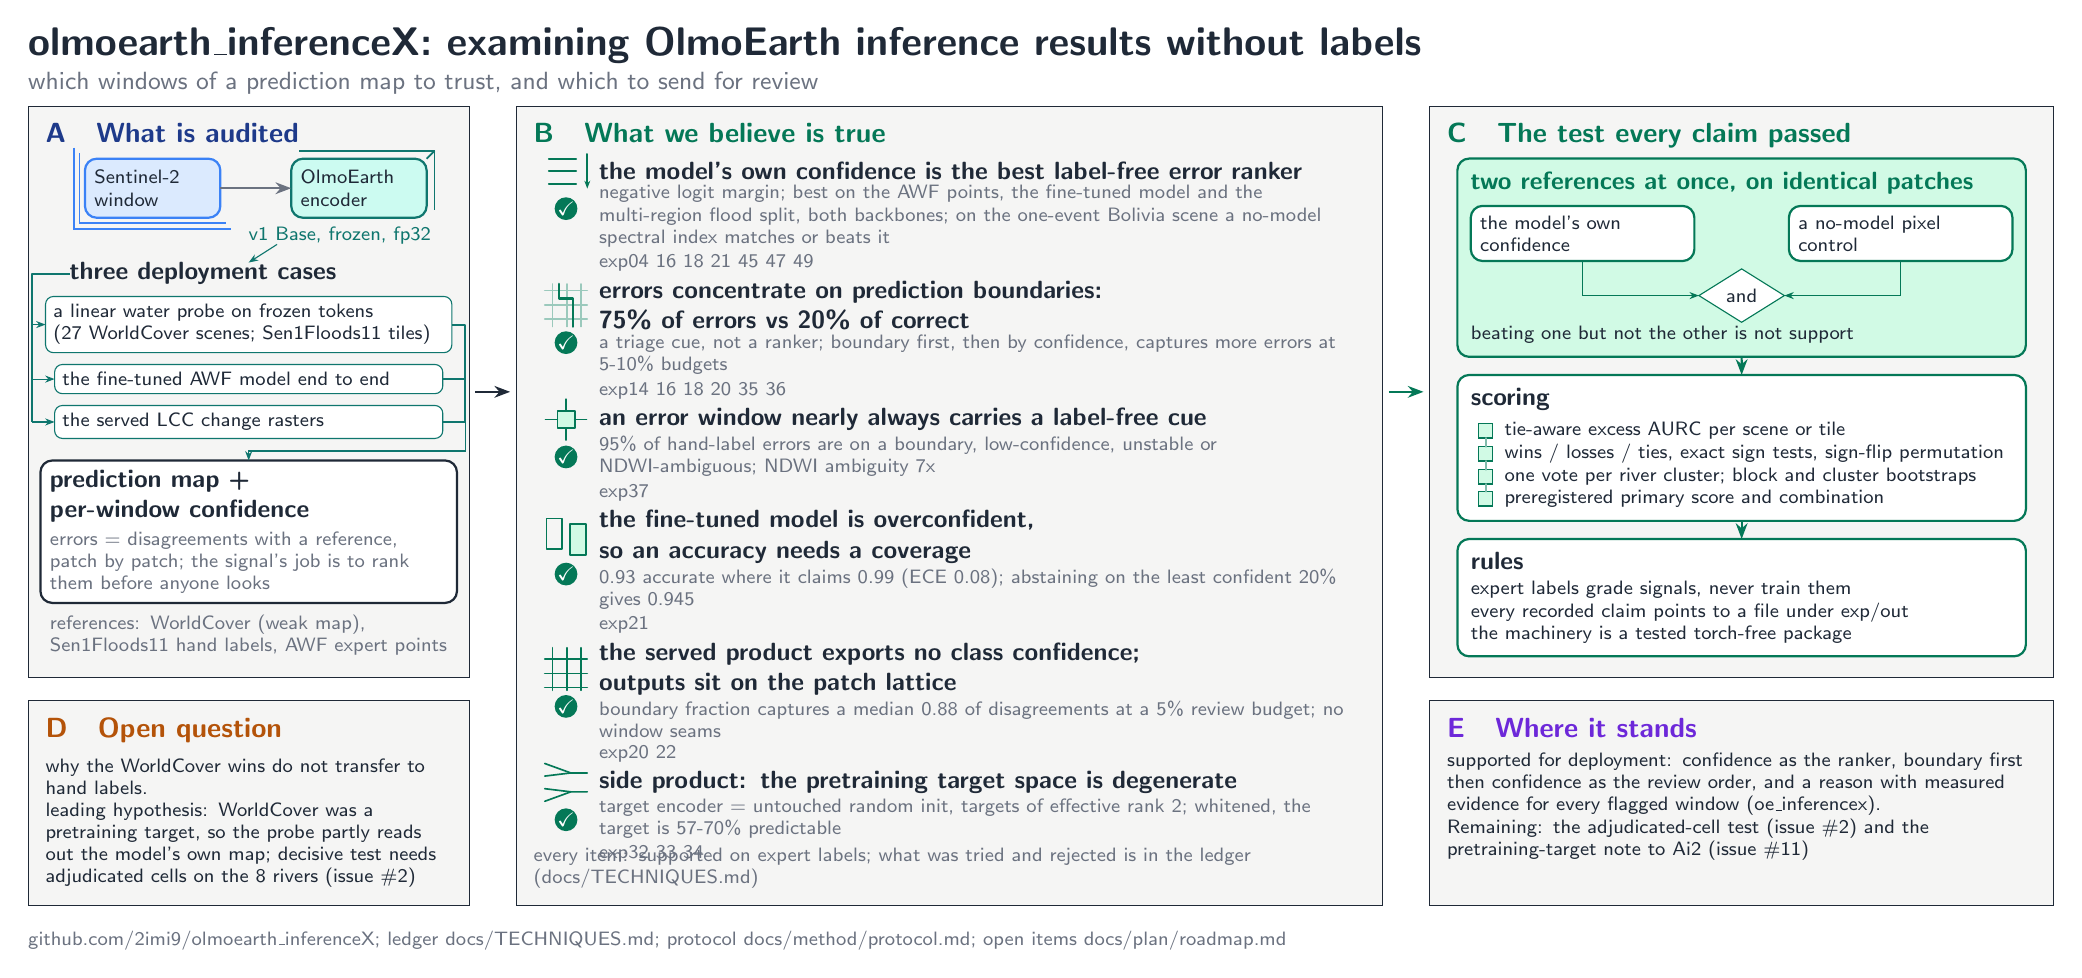
\begin{tikzpicture}[
  font=\sffamily, text=INK, node distance=2mm,
  every node/.style={inner sep=0pt, outer sep=0pt, align=left, execute at begin node=\raggedright},
  panel/.style={rectangle, draw=INK, thin, fill=PANEL, inner sep=0pt},
  box/.style={rectangle, rounded corners=1.5mm, draw=EMERALD, thick, fill=white, inner sep=2mm, align=left},
  flowbox/.style={box, inner sep=1.2mm, draw=TEAL, text width=5.05cm, font=\sffamily\scriptsize},
  claim/.style={text width=9.73cm, align=left, font=\sffamily\small\bfseries},
  evidence/.style={text width=9.73cm, align=left, font=\sffamily\scriptsize, text=MUTED},
  ids/.style={evidence},
  check/.style={circle, fill=EMERALD, text=white, minimum size=3.5mm, font=\sffamily\scriptsize\bfseries},
  arrow/.style={-{Stealth[length=2mm]}, thick, draw=MUTED},
  paneltitle/.style={font=\sffamily\normalsize\bfseries, align=left},
  body/.style={font=\sffamily\scriptsize, align=left},
  boxtitle/.style={font=\sffamily\small\bfseries, align=left},
  stage/.style={draw=TEAL, fill=white, rounded corners=1mm, inner sep=1mm, text width=4.73cm, align=left, font=\sffamily\scriptsize},
  glyph/.style={draw=EMERALD, line width=0.6pt, line cap=round, line join=round},
  glyphanchor/.style={minimum width=6mm, minimum height=6mm},
  rail/.style={draw=TEAL, line width=0.7pt, line join=round},
  reference/.style={box, fill=white, text width=2.6cm, minimum height=7mm, inner sep=1.2mm, font=\sffamily\scriptsize},
  junction/.style={diamond, draw=EMERALD, fill=white, inner sep=0.8mm, aspect=1.6, font=\sffamily\scriptsize},
  scoreline/.style={font=\sffamily\scriptsize, text width=6.45cm, align=left}
]

% Panel anchors are the only absolute coordinates. Dimensions are in cm.
\coordinate (a-nw) at (0,0);
\coordinate (b-nw) at (6.2,0);
\coordinate (c-nw) at (17.8,0);
\coordinate (d-nw) at (0,-7.55);
\coordinate (e-nw) at (17.8,-7.55);
\coordinate (a-se) at ($(a-nw)+(5.6,-7.25)$);
\coordinate (b-se) at ($(b-nw)+(11,-10.15)$);
\coordinate (c-se) at ($(c-nw)+(7.919,-7.25)$);
\coordinate (d-se) at ($(d-nw)+(5.6,-2.6)$);
\coordinate (e-se) at ($(e-nw)+(7.919,-2.6)$);

% Fit panel frames behind all content.
\begin{scope}[on background layer]
\node[panel, fit=(a-nw)(a-se)] (panel-a) {};
\node[panel, fit=(b-nw)(b-se)] (panel-b) {};
\node[panel, fit=(c-nw)(c-se)] (panel-c) {};
\node[panel, fit=(d-nw)(d-se)] (panel-d) {};
\node[panel, fit=(e-nw)(e-se)] (panel-e) {};
\end{scope}

% Title and subtitle.
\node[text width=25.719cm, align=left, font=\sffamily\Large\bfseries, above=5.5mm of a-nw, anchor=south west] (title) {olmoearth\_inferenceX: examining OlmoEarth inference results without labels};
\node[text width=25.719cm, align=left, font=\sffamily\small, text=MUTED, below=1.2mm of title.south west, anchor=north west] (subtitle) {which windows of a prediction map to trust, and which to send for review};

% A: geometric inputs, three parallel deployment cases, and a merged output.
\node[paneltitle, text=NAVY, text width=5.16cm, anchor=north west] (a-title) at ($(a-nw)+(0.22,-0.22)$) {A\quad What is audited};
\node[flowbox, fill=BLUE_L, draw=BLUE, text width=1.48cm, minimum height=7.5mm, below=2mm of a-title.south west, xshift=5mm, anchor=north west] (sentinel) {Sentinel-2\\window};
\node[flowbox, fill=TEAL_L, text width=1.48cm, minimum height=7.5mm, right=9mm of sentinel] (encoder) {OlmoEarth\\encoder};
\draw[draw=BLUE, line width=0.6pt] ($(sentinel.north west)+(-0.07,0.07)$) -- ($(sentinel.south west)+(-0.07,-0.07)$) -- ($(sentinel.south east)+(0.07,-0.07)$);
\draw[draw=BLUE, line width=0.6pt] ($(sentinel.north west)+(-0.14,0.14)$) -- ($(sentinel.south west)+(-0.14,-0.14)$) -- ($(sentinel.south east)+(0.14,-0.14)$);
\draw[draw=TEAL, line width=0.6pt] ($(encoder.north west)+(0.1,0.1)$) -- ($(encoder.north east)+(0.1,0.1)$) -- ($(encoder.south east)+(0.1,0.1)$);
\draw[draw=TEAL, line width=0.6pt] (encoder.north east) -- ($(encoder.north east)+(0.1,0.1)$);
\node[body, text=TEAL, text width=2.8cm, below=1.2mm of encoder] (version) {v1 Base, frozen, fp32};
\node[boxtitle, text width=4.55cm, below=2.3mm of version.south, xshift=-14mm] (cases-title) {three deployment cases};
\node[fit=(sentinel)(encoder)(version), inner sep=0pt] (inputs) {};
\draw[arrow, draw=TEAL, thin, -{Stealth[length=1.2mm]}] (inputs.south) -- (cases-title.north);
\node[stage, text width=4.96cm, below=1.5mm of cases-title] (case-probe) {a linear water probe on frozen tokens\\(27 WorldCover scenes; Sen1Floods11 tiles)};
\node[stage, below=1.5mm of case-probe] (case-awf) {the fine-tuned AWF model end to end};
\node[stage, below=1.5mm of case-awf] (case-lcc) {the served LCC change rasters};
\coordinate (case-fork) at ($(case-probe.west)+(-0.17,0)$);
\coordinate (case-merge) at ($(case-probe.east)+(0.17,0)$);
\draw[rail] (cases-title.west) -- (case-fork |- cases-title.west) -- (case-fork |- case-lcc.west);
\draw[arrow, draw=TEAL, thin, -{Stealth[length=1.2mm]}] (case-fork) -- (case-probe.west);
\draw[arrow, draw=TEAL, thin, -{Stealth[length=1.2mm]}] (case-fork |- case-awf.west) -- (case-awf.west);
\draw[arrow, draw=TEAL, thin, -{Stealth[length=1.2mm]}] (case-fork |- case-lcc.west) -- (case-lcc.west);
\draw[rail] (case-probe.east) -- (case-merge) -- (case-merge |- case-lcc.east) -- (case-lcc.east);
\draw[rail] (case-awf.east) -- (case-merge |- case-awf.east);
\node[boxtitle, text width=5.05cm, below=4mm of case-lcc] (prediction-title) {prediction map +\\per-window confidence};
\node[body, text=MUTED, text width=5.05cm, below=1.2mm of prediction-title] (prediction-body) {errors = disagreements with a reference,\\patch by patch; the signal's job is to rank\\them before anyone looks};
\scoped[on background layer] \node[flowbox, draw=INK, fit=(prediction-title)(prediction-body)] (prediction) {};
\coordinate (prediction-join) at ($(prediction.north)+(0,0.12)$);
\draw[arrow, draw=TEAL, thin, -{Stealth[length=1.2mm]}] (case-merge |- case-lcc.east) |- (prediction-join) -- (prediction.north);
\node[evidence, text width=5.05cm, below=1.5mm of prediction] (references) {references: WorldCover (weak map), Sen1Floods11 hand labels, AWF expert points};
\draw[arrow] (sentinel.east) -- (encoder.west);

% B: six beliefs, each with its exact evidence and experiment identifiers.
\node[paneltitle, text=EMERALD, text width=10.56cm, anchor=north west] (b-title) at ($(b-nw)+(0.22,-0.22)$) {B\quad What we believe is true};
\node[claim, below=2.5mm of b-title.south west, xshift=8.3mm, anchor=north west] (claim1) {the model's own confidence is the best label-free error ranker};
\node[evidence, below=0.7mm of claim1.south west, anchor=north west] (evidence1) {negative logit margin; best on the AWF points, the fine-tuned model and the multi-region flood split, both backbones; on the one-event Bolivia scene a no-model spectral index matches or beats it};
\node[ids, below=1mm of evidence1.south west, anchor=north west] (ids1) {exp04 16 18 21 45 47 49};
\node[glyphanchor, left=1.2mm of claim1.west] (glyph1) {};
\node[check, minimum size=2.6mm, below=0.3mm of glyph1] (check1) {$\checkmark$};
\node[claim, below=1.2mm of ids1.south west, anchor=north west] (claim2) {errors concentrate on prediction boundaries:\\75\% of errors vs 20\% of correct};
\node[evidence, below=0.7mm of claim2.south west, anchor=north west] (evidence2) {a triage cue, not a ranker; boundary first, then by confidence, captures more errors at 5-10\% budgets};
\node[ids, below=1mm of evidence2.south west, anchor=north west] (ids2) {exp14 16 18 20 35 36};
\node[glyphanchor, left=1.2mm of claim2.west] (glyph2) {};
\node[check, minimum size=2.6mm, below=0.3mm of glyph2] (check2) {$\checkmark$};
\node[claim, below=1.2mm of ids2.south west, anchor=north west] (claim3) {an error window nearly always carries a label-free cue};
\node[evidence, below=0.7mm of claim3.south west, anchor=north west] (evidence3) {95\% of hand-label errors are on a boundary, low-confidence, unstable or NDWI-ambiguous; NDWI ambiguity 7x};
\node[ids, below=1mm of evidence3.south west, anchor=north west] (ids3) {exp37};
\node[glyphanchor, left=1.2mm of claim3.west] (glyph3) {};
\node[check, minimum size=2.6mm, below=0.3mm of glyph3] (check3) {$\checkmark$};
\node[claim, below=1.2mm of ids3.south west, anchor=north west] (claim4) {the fine-tuned model is overconfident,\\so an accuracy needs a coverage};
\node[evidence, below=0.7mm of claim4.south west, anchor=north west] (evidence4) {0.93 accurate where it claims 0.99 (ECE 0.08); abstaining on the least confident 20\% gives 0.945};
\node[ids, below=1mm of evidence4.south west, anchor=north west] (ids4) {exp21};
\node[glyphanchor, left=1.2mm of claim4.west] (glyph4) {};
\node[check, minimum size=2.6mm, below=0.3mm of glyph4] (check4) {$\checkmark$};
\node[claim, below=1.2mm of ids4.south west, anchor=north west] (claim5) {the served product exports no class confidence;\\outputs sit on the patch lattice};
\node[evidence, below=0.7mm of claim5.south west, anchor=north west] (evidence5) {boundary fraction captures a median 0.88 of disagreements at a 5\% review budget; no window seams};
\node[ids, below=1mm of evidence5.south west, anchor=north west] (ids5) {exp20 22};
\node[glyphanchor, left=1.2mm of claim5.west] (glyph5) {};
\node[check, minimum size=2.6mm, below=0.3mm of glyph5] (check5) {$\checkmark$};
\node[claim, below=1.2mm of ids5.south west, anchor=north west] (claim6) {side product: the pretraining target space is degenerate};
\node[evidence, below=0.7mm of claim6.south west, anchor=north west] (evidence6) {target encoder = untouched random init, targets of effective rank 2; whitened, the target is 57-70\% predictable};
\node[ids, below=1mm of evidence6.south west, anchor=north west] (ids6) {exp32 33 34};
\node[glyphanchor, left=1.2mm of claim6.west] (glyph6) {};
\node[check, minimum size=2.6mm, below=0.3mm of glyph6] (check6) {$\checkmark$};
\node[evidence, text width=10.56cm, anchor=south east] (legend) at ($(b-se)+(-0.22,0.22)$) {every item: supported on expert labels; what was tried and rejected is in the ledger\\(docs/TECHNIQUES.md)};

% Six unscaled conceptual glyphs: ranking, boundary, cues, calibration, lattice, rank two.
\draw[glyph] ($(glyph1.west)+(0.08,0.16)$) -- ($(glyph1.east)+(-0.17,0.16)$);
\draw[glyph] ($(glyph1.west)+(0.08,0)$) -- ($(glyph1.east)+(-0.17,0)$);
\draw[glyph] ($(glyph1.west)+(0.08,-0.16)$) -- ($(glyph1.east)+(-0.17,-0.16)$);
\draw[glyph, -{Stealth[length=1mm]}] ($(glyph1.east)+(-0.03,0.22)$) -- ($(glyph1.east)+(-0.03,-0.22)$);
\draw[glyph, step=1.8mm, draw=EMERALD!40] ($(glyph2.center)+(-0.27,-0.27)$) grid ($(glyph2.center)+(0.27,0.27)$);
\draw[glyph, line width=1pt] ($(glyph2.center)+(-0.09,0.27)$) -- ($(glyph2.center)+(-0.09,0.09)$) -- ($(glyph2.center)+(0.09,0.09)$) -- ($(glyph2.center)+(0.09,-0.27)$);
\draw[glyph, fill=EMERALD_L] ($(glyph3.center)+(-0.11,-0.11)$) rectangle ($(glyph3.center)+(0.11,0.11)$);
\draw[glyph] ($(glyph3.center)+(-0.26,0)$) -- ($(glyph3.center)+(-0.11,0)$) ($(glyph3.center)+(0.11,0)$) -- ($(glyph3.center)+(0.26,0)$);
\draw[glyph] ($(glyph3.center)+(0,0.26)$) -- ($(glyph3.center)+(0,0.11)$) ($(glyph3.center)+(0,-0.11)$) -- ($(glyph3.center)+(0,-0.26)$);
\draw[glyph] ($(glyph4.center)+(-0.25,-0.16)$) rectangle ($(glyph4.center)+(-0.05,0.23)$);
\draw[glyph, fill=EMERALD_L] ($(glyph4.center)+(0.05,-0.23)$) rectangle ($(glyph4.center)+(0.25,0.16)$);
\draw[glyph, step=1.8mm] ($(glyph5.center)+(-0.27,-0.27)$) grid ($(glyph5.center)+(0.27,0.27)$);
\draw[glyph] ($(glyph6.center)+(-0.27,0.24)$) -- ($(glyph6.center)+(0.06,0.12)$) -- ($(glyph6.center)+(0.27,0.12)$);
\draw[glyph] ($(glyph6.center)+(-0.27,0.08)$) -- ($(glyph6.center)+(0.06,0.12)$);
\draw[glyph] ($(glyph6.center)+(-0.27,-0.08)$) -- ($(glyph6.center)+(0.06,-0.12)$) -- ($(glyph6.center)+(0.27,-0.12)$);
\draw[glyph] ($(glyph6.center)+(-0.27,-0.24)$) -- ($(glyph6.center)+(0.06,-0.12)$);

% C: two comparison inputs merge before scoring and rules.
\node[paneltitle, text=EMERALD, text width=7.479cm, anchor=north west] (c-title) at ($(c-nw)+(0.22,-0.22)$) {C\quad The test every claim passed};
\node[boxtitle, text=EMERALD, text width=6.879cm, below=3mm of c-title] (two-title) {two references at once, on identical patches};
\node[reference, below=1.5mm of two-title.south west, anchor=north west] (model-reference) {the model's own confidence};
\node[reference, right=12mm of model-reference] (pixel-reference) {a no-model pixel control};
\coordinate (reference-mid) at ($(model-reference.south)!0.5!(pixel-reference.south)$);
\node[junction, below=1mm of reference-mid] (and) {and};
\draw[arrow, draw=EMERALD, thin, -{Stealth[length=1.2mm]}] (model-reference.south) |- (and.west);
\draw[arrow, draw=EMERALD, thin, -{Stealth[length=1.2mm]}] (pixel-reference.south) |- (and.east);
\node[body, text width=6.879cm, below=0.5mm of and] (two-body) {beating one but not the other is not support};
\scoped[on background layer] \node[box, fill=EMERALD_L, inner sep=1.7mm, fit=(two-title)(model-reference)(pixel-reference)(and)(two-body)] (two) {};
\node[boxtitle, text width=6.879cm, below=4mm of two] (scoring-title) {scoring};
\node[scoreline, below=1.5mm of scoring-title.south west, xshift=4.3mm, anchor=north west] (score1) {tie-aware excess AURC per scene or tile};
\node[scoreline, below=0.6mm of score1.south west, anchor=north west] (score2) {wins / losses / ties, exact sign tests, sign-flip permutation};
\node[scoreline, below=0.6mm of score2.south west, anchor=north west] (score3) {one vote per river cluster; block and cluster bootstraps};
\node[scoreline, below=0.6mm of score3.south west, anchor=north west] (score4) {preregistered primary score and combination};
\node[draw=EMERALD, fill=EMERALD_L, minimum size=1.8mm, left=1.5mm of score1.west] (score-mark1) {};
\node[draw=EMERALD, fill=EMERALD_L, minimum size=1.8mm, left=1.5mm of score2.west] (score-mark2) {};
\node[draw=EMERALD, fill=EMERALD_L, minimum size=1.8mm, left=1.5mm of score3.west] (score-mark3) {};
\node[draw=EMERALD, fill=EMERALD_L, minimum size=1.8mm, left=1.5mm of score4.west] (score-mark4) {};
\draw[glyph, draw=EMERALD!50] (score-mark1.south) -- (score-mark2.north) (score-mark2.south) -- (score-mark3.north) (score-mark3.south) -- (score-mark4.north);
\scoped[on background layer] \node[box, inner sep=1.7mm, fit=(scoring-title)(score1)(score2)(score3)(score4)] (scoring) {};
\node[boxtitle, text width=6.879cm, below=4mm of scoring] (rules-title) {rules};
\node[body, text width=6.879cm, below=1.5mm of rules-title] (rules-body) {expert labels grade signals, never train them\\every recorded claim points to a file under exp/out\\the machinery is a tested torch-free package};
\scoped[on background layer] \node[box, inner sep=1.7mm, fit=(rules-title)(rules-body)] (rules) {};
\draw[arrow, draw=EMERALD] (two.south) -- (scoring.north);
\draw[arrow, draw=EMERALD] (scoring.south) -- (rules.north);

% D: open question and next step.
\node[paneltitle, text=AMBER, text width=5.16cm, anchor=north west] (d-title) at ($(d-nw)+(0.22,-0.22)$) {D\quad Open question};
\node[body, text width=5.16cm, below=2mm of d-title] (d-body) {why the WorldCover wins do not transfer to hand labels.\\leading hypothesis: WorldCover was a pretraining target, so the probe partly reads out the model's own map; decisive test needs adjudicated cells on the 8 rivers (issue \#2)};

% E: deployment status and remaining work.
\node[paneltitle, text=VIOLET, text width=7.479cm, anchor=north west] (e-title) at ($(e-nw)+(0.22,-0.22)$) {E\quad Where it stands};
\node[body, text width=7.479cm, below=2mm of e-title] (e-body) {supported for deployment: confidence as the ranker, boundary first then confidence as the review order, and a reason with measured evidence for every flagged window (oe\_inferencex).\\Remaining: the adjudicated-cell test (issue \#2) and the pretraining-target note to Ai2 (issue \#11)};

% Inter-panel arrows share the midpoint of the upper panels.
\coordinate (ab-start) at ($(panel-a.east)+(0.08,0)$);
\coordinate (ab-end) at ($(panel-b.west |- ab-start)+(-0.08,0)$);
\coordinate (bc-end) at ($(panel-c.west)+(-0.08,0)$);
\coordinate (bc-start) at ($(panel-b.east |- bc-end)+(0.08,0)$);
\draw[arrow, draw=INK] (ab-start) -- (ab-end);
\draw[arrow, draw=EMERALD] (bc-start) -- (bc-end);

% Source footer.
\node[evidence, text width=25.719cm, below=3.2mm of panel-d.south west, anchor=north west] (footer) {github.com/2imi9/olmoearth\_inferenceX; ledger docs/TECHNIQUES.md; protocol docs/method/protocol.md; open items docs/plan/roadmap.md};
\end{tikzpicture}
\end{document}
